%%==================================================
%% chapter01.tex for BIT Master Thesis
%% modified by yang yating
%% version: 0.1
%% last update: Dec 25th, 2016
%%==================================================
\chapter{Introduction}
\label{chap:INTRODUCTION}
\section{Reseach Background}
The interplay between global commerce and environmental sustainability has escalated into a prominent area of scholarly investigation, reflecting the growing complexity of international trade's impact on ecological systems (\supercitet{RN123}; \supercitet{RN166}). In the wake of increasing global interconnectedness, 2022 saw international trade account for more than 30\% of global GDP, while also contributing significantly to global carbon emissions—exceeding one-quarter of the total emissions (\supercitet{RN176}). This significant environmental footprint underscores the urgent need to explore the mechanisms through which global trade practices distribute pollutants across regions, particularly highlighting stark disparities in pollution levels between developed and developing nations (\supercitet{RN133}; \supercitet{RN161}).

Historically, the relocation of pollution-intensive industries from developed to less regulated developing regions has been perceived as a strategic move to circumvent stringent environmental laws, thereby raising critical questions about the actual environmental cost of free trade. This shift not only exacerbates the emission levels in developing regions but also complicates the global efforts to mitigate environmental impacts (\supercitet{RN169}). The global trade environment is further complicated by recent geopolitical events, including intensifying trade frictions between major economies such as the U.S. and China, Brexit implications, the establishment of regional trade barriers (\supercitet{RN160}), and significant policy enactments like the U.S. export controls. The onset of the 2020 pandemic added another layer of complexity, propelling nations towards an unprecedented level of protectionism characterized by severe trade restrictions (\supercitet{RN143}; \supercitet{RN111}).

Focusing on the U.S.-China trade dynamics as detailed in Table \ref{tab:timeline}, this research seeks to dissect the environmental outcomes of these economic interactions. As the two largest global economies and leading carbon emitters, the trade activities between these nations not only shape economic landscapes but also significantly influence global environmental policies and practices. In 2019, the U.S. and China accounted for 28\% and 14\% of global CO2 emissions respectively, with their bilateral trade constituting a significant portion of the world trade (\supercitet{RN180}). The recent trade disputes, marked by the U.S.'s CHIPS and Science Act and China's strategic export controls, offer a compelling case study to explore the environmental ramifications of these economic engagements.

The semiconductor industry occupies a unique position within the U.S.-China trade landscape, characterized by its high technological intensity and strategic significance. This sector not only drives significant economic value but also acts as a focal point in the technological rivalry between these two global powers. The intricacies of semiconductor trade between the U.S. and China are highlighted by the frequent shifts in policy, ranging from the U.S. imposing restrictions on semiconductor exports to China, to China's maneuvers to bolster its domestic chip manufacturing capabilities in response (\supercitet{RN180}). These dynamics are critical as they not only influence trade policies but also affect global supply chains and innovation trajectories in technology-intensive sectors.

The environmental impacts of this trade are multifaceted. On one hand, the advanced technologies used in semiconductor manufacturing require substantial resources, including water and energy, and involve the use of hazardous chemicals, which pose significant environmental risks if not managed properly (\supercitet{RN176}). On the other hand, the drive towards more advanced semiconductor technologies can lead to more energy-efficient products, potentially mitigating some of the environmental impacts associated with electronic devices' life cycles. However, the escalation of trade tensions and the resulting shifts in production locations may lead to environmental deregulation as countries compete for manufacturing dominance. This scenario can exacerbate the environmental costs in regions that may adopt less stringent environmental controls to attract or retain semiconductor manufacturing facilities. Thus, understanding the environmental outcomes of semiconductor trade requires a nuanced approach, considering both the direct impacts of manufacturing and the broader implications of global trade policies on environmental standards and practices.

This enriched backdrop serves as the foundation for this study, aiming to provide an in-depth analysis of how shifts in global trade policies, particularly those influenced by major geopolitical events, affect environmental outcomes. Through this lens, the research will examine the broader implications of international trade on global sustainability efforts, making it crucial to understand and possibly reframe the ongoing discourse on trade and environment in the contemporary global economy.

\begin{table}
     \centering
     \caption{U.S. and China Relationship in the context of trade tension timeline} \label{tab:timeline}
     \begin{tabular}{|p{0.1\textwidth}|p{0.9\textwidth}|}
     \toprule
       Year & Event \\
     \midrule
       2000 & Normalization of trade relations between the U.S. and China. \\
       2008 & China becomes the largest U.S. foreign creditor. \\
       2010 & China becomes the world's second-largest economy. \\
       2011 & U.S. 'pivots' toward Asia, countering China's growing clout, and announces the Trans-Pacific Partnership. \\
       2012 & Rising U.S.-China trade tensions, with the U.S. trade deficit with China reaching an all-time high of \$295.5 billion. \\
       2013 & Sunnylands Summit between U.S. and China leaders. \\
       2016 & China aims to reduce energy intensity by 15\% under its 13th Five-Year Plan. \\
       2017 & China commits to investing \$360 billion in renewable energy by 2020, reducing coal reliance. \\
       2018 & The U.S. imposes tariffs on Chinese goods, marking the beginning of the U.S.-China trade war. \\
       2020 & China leads in renewable energy, investing in solar panels and wind turbines. \\
            & The 'Phase One' trade deal is signed amid rising tensions due to the COVID-19 pandemic. \\
            & The U.S. imposes restrictions on China's semiconductor industry. \\
            & Huawei faces severe U.S. restrictions, leading to a substantial revenue decline. \\
            & China already has \$150 billion in chip subsidies. \\
       2021 & Biden administration enhances restrictions on China's semiconductor industry. \\
       2022 & The U.S. Congress passes the CHIPS and Science Act, providing subsidies and tax breaks to boost domestic semiconductor production. \\
            & Additional sanctions are imposed on Chinese companies, and the entity list of restricted companies expands significantly. \\
            & The National Defense Authorization Act prohibits U.S. government agencies from procuring products containing semiconductors made by China's leading chip manufacturers. \\
            & Huawei's partner, SMIC, achieves a breakthrough in 7nm chip manufacturing. \\
            & Japan announces restrictions on exporting 23 types of equipment used in chip-making processes to China. \\
            & President Xi Jinping announces the New Whole Nation System for self-reliance in critical national security technologies. \\
       2023 & China introduces a new export license system for gallium and germanium. \\
            & The Netherlands limits exports to China of deep ultraviolet lithography machines. \\
            & U.S. restricts export of cutting-edge chips and chip-making equipment to China. \\
            & The U.S. implements the Advanced Computing Chips Rule and the Expansion of Export Controls on Semiconductor Manufacturing Items Interim Final Rule. \\
            & Introduction of two new Temporary General Licenses (TGLs). \\
            & Huawei launches Mate 60 and Mate 60 Pro with HiSilicon Kirin 9000S processors. \\
            & U.S. Commerce Department finalizes guardrails limiting expansion in China for companies receiving subsidies under the 2022 CHIPS and Science Act. \\
            & China upgrades its semiconductor R\&D tax credit by 20\%. \\
   \bottomrule
   \end{tabular}
   \end{table}
   
\section{Research Content}

This study delves into the intricate dynamics of trade protectionism and its environmental repercussions, particularly focusing on the semiconductor industry and its significant role within the broader framework of global trade and carbon emissions. Utilizing the extensive dataset from Exiobase3 covering the period from 2000 to 2022, the research adopts a nuanced methodological approach that goes beyond traditional binary analyses of trade scenarios. Instead, it explores a graduated range of trade restriction scenarios to provide a more detailed understanding of their environmental impacts.

The research is structured around several key investigative areas. Initially, the study quantifies the carbon emissions linked to the semiconductor trade, employing the MRIO model to map out the flow of goods and associated emissions across international boundaries. This step is crucial in understanding the primary sources of emissions and the extent to which trade can influence global carbon footprints. By comparing actual trade scenarios with hypothetical no-trade conditions, the research highlights the significant role trade policies play in shaping environmental outcomes.

Moreover, the research employs a sophisticated cooperative game theoretical framework to analyze the complex effects of trade protectionism across different nations. This approach allows for an in-depth exploration of how trade policies influence global CO2 emissions, bridging the gap between economic activities and environmental outcomes. The game-theoretical model facilitates an understanding of the strategic interactions among nations, considering both competitive and cooperative behaviors in the global trade arena.

The primary objective of this research is to provide a profound comprehension of the complex interplay between trade policies and environmental sustainability. It seeks to uncover the nuanced implications of trade protectionism, particularly in technologically advanced sectors, against the backdrop of ongoing trade conflicts between the United States and China. The study aims to offer insights into how current and future trade policies might shape global environmental sustainability, especially in terms of carbon emissions, within the increasingly globalized economic landscape.

By advancing these methodological innovations and analytical frameworks, the research contributes significantly to the academic discourse on trade and environment. It provides policymakers and scholars with a deeper understanding of how trade dynamics influence environmental outcomes, emphasizing the need for integrated approaches to managing trade and environmental policies in a way that supports sustainable global development.

\section{Research Significance}
The significance of this research extends across both theoretical and practical dimensions, contributing profoundly to the discourse on trade, technology, and environmental sustainability. Theoretically, this study enhances the application of multi-regional input-output (MRIO) models and cooperative game theoretical frameworks within the context of international trade and environmental impacts. By integrating these sophisticated methodologies, the research enriches the analytical approaches available for examining the environmental consequences of trade policies. This theoretical advancement not only broadens the scope of economic models in environmental studies but also introduces a nuanced perspective on the interplay between trade dynamics and global sustainability efforts.

From a practical standpoint, the findings of this research hold substantial implications for policymakers and industry stakeholders. By demonstrating the environmental benefits of current trade structures, particularly within the semiconductor industry, the study provides essential insights that can inform policy decisions. The detailed analysis of carbon emission shifts under various trade scenarios offers a valuable tool for governments and international organizations to assess the potential outcomes of trade policies on environmental sustainability. This is particularly pertinent in the context of ongoing global discussions about trade agreements and environmental regulations.

Furthermore, the insights derived from this research regarding the semiconductor industry's role in global carbon emissions are critically important for industry stakeholders. As semiconductor manufacturing is both energy-intensive and central to modern technology, understanding its impact on carbon emissions is crucial for developing more sustainable production practices. The data-driven insights provided by this study could guide the semiconductor industry in adopting greener technologies and practices that align with global carbon reduction goals.

In summary, the research not only contributes to academic knowledge by applying and expanding upon advanced methodological frameworks but also serves as a strategic guide for policymakers and industry leaders. By elucidating the complex relationship between trade policies and environmental outcomes, it supports informed decision-making that could lead to more effective environmental strategies and trade agreements. This dual contribution underscores the relevance and urgency of integrating economic and environmental considerations in the planning and implementation of trade policies worldwide.


\section{Thesis Structure}

This thesis is meticulously organized into five chapters, each delineating a distinct aspect of the study, designed to provide a comprehensive understanding of the interplay between trade policies and environmental impacts, with a specific focus on the semiconductor industry.

\textbf{Chapter 1 Introduction} sets the stage for the research by presenting the background, which articulates the relevance of exploring the environmental implications of global trade, particularly within the context of rising trade protectionism and technological advancements in semiconductor production. The research content, significance, and a detailed structure of the thesis are also outlined, providing a clear roadmap for the reader.

\textbf{Chapter 2 Literature Review} explores existing scholarly work related to the environmental consequences of international trade, with an emphasis on input-output analysis. This chapter is divided into four sections, each reviewing different aspects of the literature that discuss environmental impacts from trade, the dual outcomes of trade frictions, specific issues concerning the semiconductor industry, and new paradigms in assessing the impact of global production-based redistribution. This comprehensive review helps to position the current study within the existing body of knowledge and identifies gaps that the research aims to fill.

\textbf{Chapter 3 Methodology and Data} describes the analytical frameworks and data sources used in this study. It begins with a detailed explanation of the MRIO model employed to calculate trade-related variables and assess carbon footprints. The chapter progresses to discuss the unique scenarios modeled in this study, including no-trade conditions, and concludes with the methodologies used for data collection, primarily focusing on the use of Exiobase3. This methodological groundwork is essential for understanding the subsequent analysis of trade impacts on global carbon emissions.

\textbf{Chapter 4 Empirical Results} presents the findings from the application of the methodologies described in Chapter 3. This chapter is structured to sequentially address the research questions posed, analyzing the global carbon emissions related to international trade, the differences between production-based and consumption-based accounting of emissions, and the specific impacts of semiconductor trade under various hypothetical trade scenarios. Detailed analysis of the semiconductor industry's upstream and downstream impacts on global carbon emissions is also provided. This chapter is crucial as it translates the theoretical and methodological frameworks into practical insights.

\textbf{Chapter 5 Conclusions and Policy Recommendations} synthesizes the findings from the empirical analysis, highlighting the nuanced implications of trade protectionism on carbon emissions globally. The chapter offers concrete policy recommendations based on the research findings, aimed at optimizing trade practices to enhance global environmental outcomes. It also reflects on the broader implications of these findings for policymakers, industry stakeholders, and the academic community.

Throughout the thesis, references and appendices provide additional support and resources, including detailed descriptions of semiconductivity-related products and a list of ISO 3166-1 country codes, which assist in understanding the technical aspects and geographical scope of the research. This structured approach ensures a logical flow of information, facilitating a thorough understanding of the complex relationships between trade and environmental sustainability.

\ifincludefigures
\begin{figure}
\centering
\makebox[\textwidth][c]{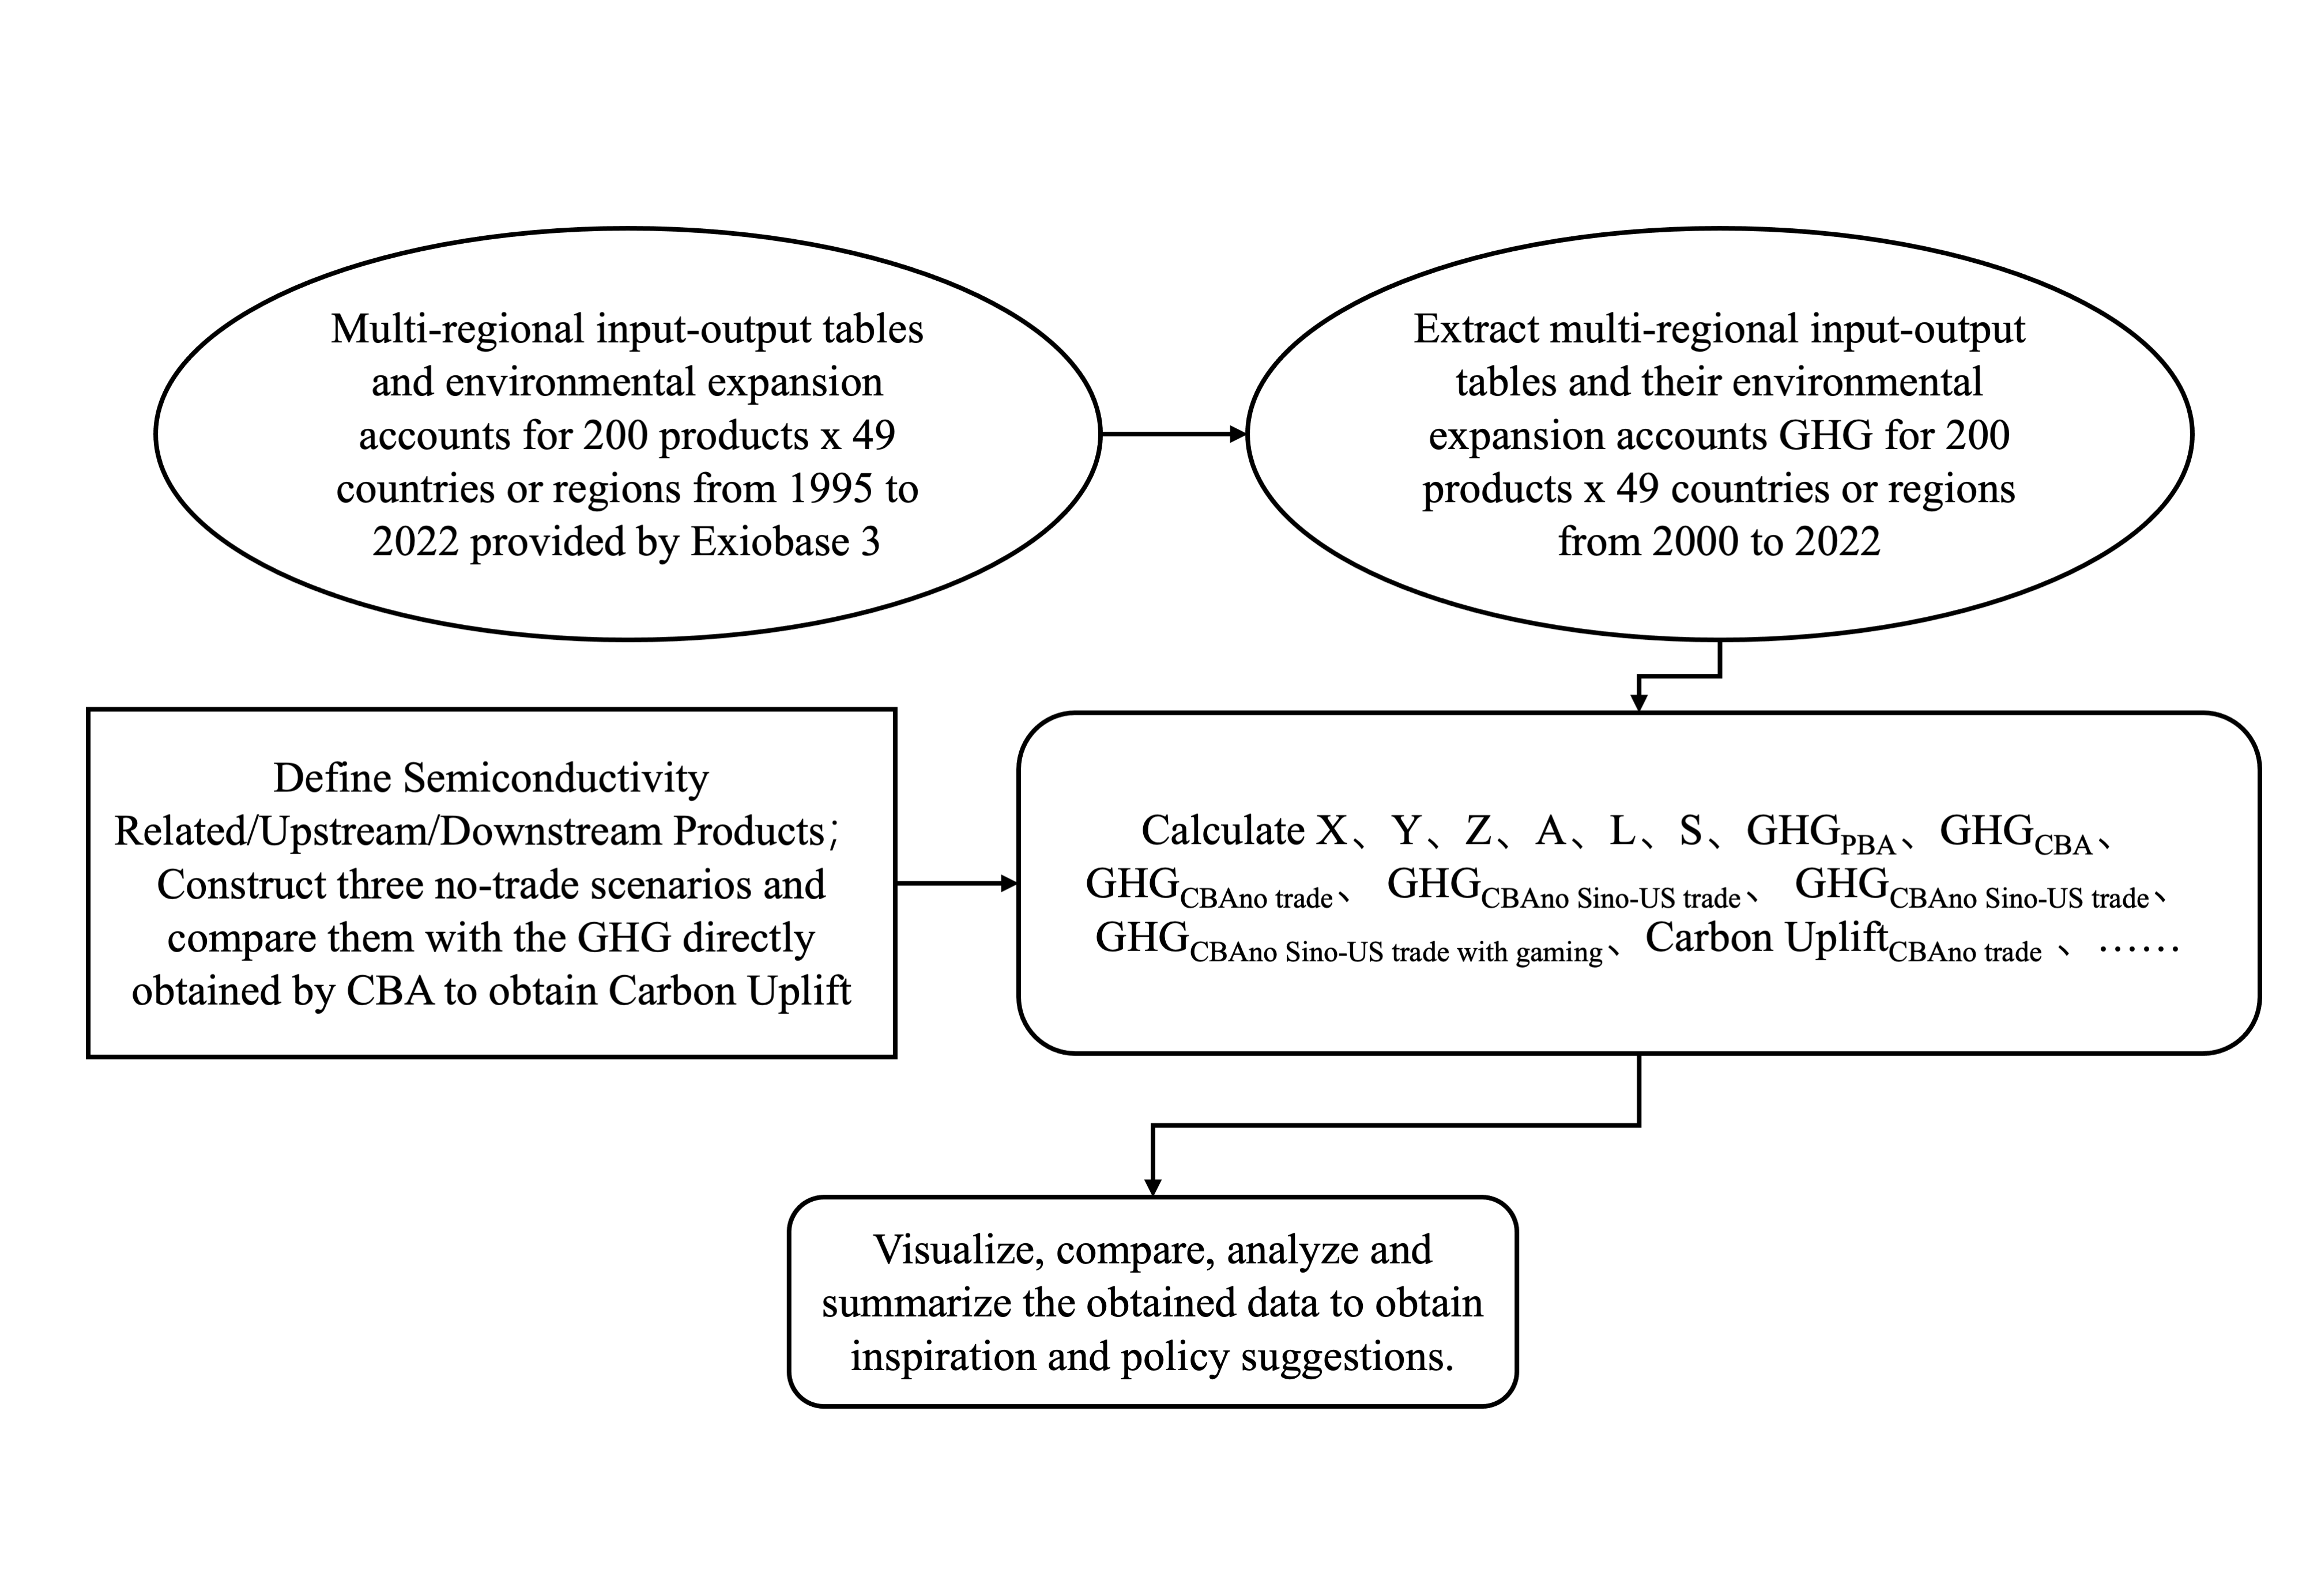
\includegraphics[width=1\textwidth]{figures/Graph/幻灯片2.png}}
 \caption{Technical Roadmap}\label{fig:tech roadmap}
\end{figure}
\fi                                                                                                                                                                                     
Figure \ref{fig:tech roadmap} illustrates the structured methodology employed in this thesis to analyze the environmental impacts of international trade, with a specific focus on the semiconductor industry, utilizing multi-regional input-output (MRIO) tables and environmental expansion accounts provided by Exiobase 3. The approach is divided into several key stages to ensure a comprehensive assessment of the trade-related carbon footprint.

Initially, the study extracts MRIO tables and their corresponding environmental data covering the years 2000 to 2022 for 200 products across 49 countries or regions. This extensive data extraction forms the basis for all subsequent analyses, offering a detailed and expansive perspective on global trade and environmental interactions.

Following data extraction, the study defines specific product categories related to semiconductivity, including upstream and downstream products. These categories are crucial for focusing the analysis on relevant sectors within the semiconductor industry. The research constructs three distinct no-trade scenarios to simulate the environmental impacts in the absence of trade. These scenarios are compared with actual greenhouse gas emissions data obtained through consumption-based accounting (CBA), allowing for a nuanced calculation of carbon uplift due to trade activities.

The core analytical phase involves calculating various elements such as total output ($X$), intermediate inputs ($Z$), final demand ($Y$), and the Leontief inverse matrix ($L$), which are foundational to understanding the economic interconnections within the MRIO framework. These calculations lead to the estimation of greenhouse gas emissions under different trade scenarios, including no-trade, no Sino-US trade, and a scenario incorporating gaming trade redistribution, which offers insights into potential changes in carbon emissions patterns due to strategic alterations in trade policies.

The final stage of the methodology involves a detailed visualization, comparison, and analysis of the data to draw meaningful conclusions and generate policy recommendations. This process not only elucidates the quantitative impacts of trade on carbon emissions but also provides a solid empirical foundation for suggesting strategic interventions to optimize trade practices for better environmental outcomes.

The technical roadmap, as visualized in Figure \ref{fig:tech roadmap}, is integral to demonstrating the systematic approach taken in this thesis to address the complex interplay between trade and environmental policies. This structured methodology ensures that the findings are robust, comprehensive, and relevant to policymakers and industry stakeholders engaged in navigating the challenges of sustainable international trade.